\def\documentauthor{Carlos Salinas}
\def\documenttitle{MA557 Problem Set \hwnum}
\def\hwnum{3}
\def\shorttitle{MA557 PSet \hwnum}
\def\coursename{MA557}
\def\documentsubject{commutative algebra i}
\def\authoremail{salinac@purdue.edu}

\documentclass[article,oneside,10pt]{memoir}
\usepackage{geometry}
\usepackage[dvipsnames]{xcolor}
\usepackage[
    breaklinks,
    bookmarks=true,
    colorlinks=true,
    pageanchor=false,
    linkcolor=black,
    anchorcolor=black,
    citecolor=black,
    filecolor=black,
    menucolor=black,
    runcolor=black,
    urlcolor=black,
    hyperindex=false,
    hyperfootnotes=true,
    pdftitle={\shorttitle},
    pdfauthor={\documentauthor},
    pdfkeywords={\documentsubject},
    pdfsubject={\coursename}
    ]{hyperref}

\usepackage{graphicx}
\graphicspath{{figures/}}

% Misc
\usepackage{microtype}
\usepackage{multicol}
\usepackage[inline]{enumitem}
\usepackage{listings}
\usepackage{mleftright}
\mleftright

%% Math
\usepackage{amsthm}
\usepackage{amssymb}
\usepackage{mathtools}

%% PDFTeX specific
\usepackage{iftex}
\ifPDFTeX
\usepackage[mathcal]{euscript}
\usepackage{mathrsfs}

\usepackage{cmap}
\usepackage[T2A,T1]{fontenc}
\usepackage[utf8]{inputenc}
\usepackage[french,german,russian,spanish,english]{babel}
\babeltags{fr=french,
           de=german,
           ru=russian,
           es=spanish,
           en=english}
\def\spanishoptions{mexico}
\usepackage{CJKutf8}
\newcommand{\textha}[1]{\begin{CJK}{UTF8}{mj}#1\end{CJK}}
\newcommand{\textni}[1]{\begin{CJK}{UTF8}{min}#1\end{CJK}}
\newcommand{\textzh}[1]{\begin{CJK}{UTF8}{bsmi}#1\end{CJK}}
\fi

% %% XeTeX specific
% \ifXeTeX
% \usepackage{unicode-math}

% \setmainfont[Ligatures=TeX]{Latin Modern Roman}
% \setsansfont[Ligatures=TeX]{Latin Modern Sans}
% \setmonofont{Latin Modern Mono}
% \setmathfont{Latin Modern Math}

% % \usepackage{unicode-minionmath}
% % \setmainfont[Ligatures=TeX]{Minion Pro}
% % \setsansfont[Ligatures=TeX]{Myriad Pro}
% % \setmonofont[Scale=.85]{Courier Std}

% % \setmathfont{Minion Math}
% % \setmathfont[range={\mathfrak}]{XITS Math}
% % \setmathfont[range={\mathcal},StylisticSet=1]{XITS Math}
% % \setmathfont[range={\mathscr}]{XITS Math}
% % \setmathfont[range={}]{Minion Math}
% \fi

%% Theorems and definitions
\theoremstyle{plain}
\newtheorem{theorem}{Theorem}
\newtheorem{proposition}[theorem]{Proposition}
\newtheorem{corollary}[theorem]{Corollary}
\newtheorem{claim}[theorem]{Claim}
\newtheorem{lemma}[theorem]{Lemma}
\newtheorem{axiom}[theorem]{Axiom}

\newtheorem*{corollary*}{Corollary}
\newtheorem*{claim*}{Claim}
\newtheorem*{lemma*}{Lemma}
\newtheorem*{proposition*}{Proposition}
\newtheorem*{theorem*}{Theorem}

\theoremstyle{definition}
\newtheorem{definition}{Definition}
\newtheorem{example}{Examples}
\newtheorem{examples}[example]{Examples}
% \newtheorem{exercise}{Exercise}[section]
% \newtheorem{problem}[exercise]{Problem}

\newcounter{problem}
\newenvironment{problem}[1][]% environment name
{% begin code
  \stepcounter{problem}
  \par\vspace{\baselineskip}\noindent
  \ifx &#1&%
  {\normalfont\Large\bfseries\scshape Problem~\hwnum.\theproblem}
  \global\def\exercisename{Problem~\hwnum.\theproblem}%
  \else
  {\normalfont\Large\bfseries\scshape Problem~\hwnum.\theproblem~(#1)}
  \global\def\exercisename{Problem~\hwnum.\theproblem(#1)}
  \fi
  \par\vspace{\baselineskip}%
  \noindent\ignorespaces
}%
{% end code
  \par\vspace{\baselineskip}%
  \noindent\ignorespacesafterend
}

\newtheorem*{definition*}{Definition}
\newtheorem*{example*}{Examples}
\newtheorem*{examples*}{Examples}
\newtheorem*{exercise*}{Exercise}
\newtheorem*{problem*}{Problem}

\theoremstyle{remark}
\newtheorem{remark}{Remark}
\newtheorem{remarks}[remark]{Remarks}
\newtheorem{observation}[remark]{Observation}
\newtheorem{observations}[remark]{Observations}

\newtheorem*{remark*}{**Remark**}
\newtheorem*{remarks*}{**Remarks**}
\newtheorem*{observation*}{**Observation**}
\newtheorem*{observations*}{**Observations**}

%% Redefinitions & commands
\newcommand\restr[2]{{% we make the whole thing an ordinary symbol
  \left.\kern-\nulldelimiterspace % automatically resize the bar with \right
  {#1} % the function
  % \vphantom{\big|} % pretend it's a little taller at normal size
  \right|{#2} % this is the delimiter
  }}

\ifPDFTeX
\newcommand{\nsubset}{\ensuremath{\not\subset}}
\newcommand{\hooklongrightarrow}{\lhook\joinrel\longrightarrow}
\newcommand{\twoheadlongrightarrow}{\relbar\joinrel\twoheadrightarrow}

\renewcommand\qedsymbol{\ensuremath{\null\hfill\blacksquare}}

%% upint and loint
\def\upint{\mathchoice%
    {\mkern13mu\overline{\vphantom{\intop}\mkern7mu}\mkern-20mu}%
    {\mkern7mu\overline{\vphantom{\intop}\mkern7mu}\mkern-14mu}%
    {\mkern7mu\overline{\vphantom{\intop}\mkern7mu}\mkern-14mu}%
    {\mkern7mu\overline{\vphantom{\intop}\mkern7mu}\mkern-14mu}%
  \int}
\def\lowint{\mkern3mu\underline{\vphantom{\intop}\mkern7mu}\mkern-10mu\int}
\fi

% \ifXeTeX
% %% Patch arrows for XeTeX
% \usepackage{etoolbox}
% \makeatletter
% \patchcmd{\arrowfill@}{-7mu}{-14mu}{}{}
% \patchcmd{\arrowfill@}{-7mu}{-14mu}{}{}
% \patchcmd{\arrowfill@}{-2mu}{-4mu}{}{}
% \patchcmd{\arrowfill@}{-2mu}{-4mu}{}{}
% \makeatother

% \renewcommand\qedsymbol{\ensuremath{\null\hfill\QED}}
% \fi

%% Commands and operators
\DeclareMathOperator{\ann}{ann}
\DeclareMathOperator{\ass}{ass}
\DeclareMathOperator{\End}{end}
\DeclareMathOperator{\coker}{coker}
\DeclareMathOperator{\id}{id}
\DeclareMathOperator{\im}{im}
\DeclareMathOperator{\lcm}{lcm}
\DeclareMathOperator{\nil}{nil}
\DeclareMathOperator{\rad}{rad}

\newcommand{\CC}{\mathbf{C}}
\newcommand{\NN}{\mathbf{N}}
\newcommand{\QQ}{\mathbf{Q}}
\newcommand{\RR}{\mathbf{R}}
\newcommand{\ZZ}{\mathbf{Z}}

% Renewcommands
\renewcommand\setminus{\smallsetminus}
\renewcommand\phi{\varphi}
\renewcommand\epsilon{\varepsilon}

\begin{document}
\frontmatter
\aliaspagestyle{title}{empty}
\pagestyle{title}
\author{\href{mailto:\authoremail}{\documentauthor}}
\title{\documenttitle}
\date{\today}
\maketitle
\cleartooddpage

\makeoddhead{headings}
        {\small{\MakeUppercase{\itshape\documentauthor}}}
        {}
        {\small{\MakeUppercase{\itshape\exercisename}}}
\makeoddfoot{headings}{{\itshape\documenttitle}}
                      {}
                      {\thepage}
\makeevenhead{headings}
        {\small{\MakeUppercase{\itshape\documentauthor}}}
        {}
        {\small{\MakeUppercase{\itshape\exercisename}}}
\makeevenfoot{headings}{{\itshape\documenttitle}}
                      {}
                      {\thepage}
\makeheadrule{headings}{\textwidth}{.25pt}
% \makerunningwidth{headings}{1.15\textwidth}
\pagestyle{headings}

\mainmatter
\begin{problem}
Find an example of a finitely generated ring extension $R\subset
S$ where $S$ is a Noetherian ring, but $R$ is not.
\end{problem}
\begin{proof}
\end{proof}
\newpage
\begin{problem}
Consider the homomorphism of rings
\begin{center}
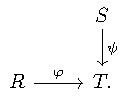
\includegraphics{figures/hw-4-ring-maps}
\end{center}
The \emph{fiber product} of $R$ and $S$ over $T$ is the subring
$R\times_T S=\left\{\,(r,s)\;\middle|\;\phi(t)=\psi(s)\,\right\}$
of $R\times S$. Assume $\phi$ and $\psi$ are surjective. Show
that if $R$ and $S$ are Noetherian rings then so is $R\times_T
S$.
\end{problem}
\begin{proof}
\end{proof}
\newpage
\begin{problem}
Let $M$ be an $R$-module. Show that $M$ is a flat $R$-module if
and only if $M_{\mathfrak{m}}$ is a flat
$R_{\mathfrak{m}}$-module for every maximal ideal $\mathfrak{m}$
of $R$.
\end{problem}
\begin{proof}
\end{proof}
\newpage
\begin{problem}
Let $M$ be an $R$-module and $\mathfrak{a}$ an $R$-ideal.
\begin{enumerate}[noitemsep,label=(\alph*)]
\item Show that if $M_{\mathfrak{m}}=0$ for every maximal ideal
  $\mathfrak{m}$ containing $\mathfrak{a}$, then $M=IM$.
\item Show that the converse holds in case $M$ is finite.
\end{enumerate}
\end{problem}
\begin{proof}
\end{proof}
\newpage
\begin{problem}
Prove that every power of a maximal ideal is primary.
\end{problem}
\begin{proof}
\end{proof}
\newpage
\begin{problem}
\begin{enumerate}[noitemsep,label=(\alph*)]
\item Show that the radical of a primary ideal is prime.
\item Find an example of a power of a prime ideal that is not
  primary.
\item Let $\mathfrak{p}$ be a prime ideal of a ring $R$ and
  $n\in\NN$. The $R$-ideal
  $\mathfrak{p}^{(n)}=R\cap\mathfrak{p}^nR_{\mathfrak{p}}$ s
  called the \emph{$n$th symbolic power of $\mathfrak{p}$}. Show
  that $\mathfrak{p}^{(n)}$ is primary.
\end{enumerate}
\end{problem}
\begin{proof}
\end{proof}

%%% Local Variables:
%%% mode: latex
%%% TeX-master: "../MA557-HW-Current"
%%% End:

\end{document}

%%% Local Variables:
%%% mode: latex
%%% TeX-master: t
%%% End:
